% latex article template

% cheat sheet(eng): http://www.pvv.ntnu.no/~walle/latex/dokumentasjon/latexsheet.pdf
% cheat sheet2(eng): http://www.pvv.ntnu.no/~walle/latex/dokumentasjon/LaTeX-cheat-sheet.pdf
% reference manual(eng): http://ctan.uib.no/info/latex2e-help-texinfo/latex2e.html

% The document class defines the type of document. Presentation, article, letter, etc. 
\documentclass[12pt, a4paper]{article}

% packages to be used. needed to use images and such things. 
\usepackage[pdfborder=0 0 0]{hyperref}
\usepackage[utf8]{inputenc}
\usepackage[english]{babel}
\usepackage{graphicx}
\PassOptionsToPackage{hyphens}{url}

% hides the section numbering. 
\setcounter{secnumdepth}{-1}

% Graphics/image lications and extensions. 
\DeclareGraphicsExtensions{.pdf, .png, .jpg, .jpeg}
\graphicspath{{./images/}}

% Title or header for the document. 
\title{
IT3010, Exercise 3
}
% Author
\author{
	Magnus L. Kirø \\
}
\date{\today}

\begin{document}
\maketitle
\pagenumbering{arabic}

\begin{abstract}
4.5 pages. 
Research Questions:

1: In which circumstance student use mobile apps for educational purpose?

2: What kind of educational activities has been done with mobile apps?

3: What kind of impacts does mobile apps has on student academic life?
\end{abstract}

\section{Data Analysis Description} %1page, 450 words
% provide 1 A4 sample page of how you do coding and grouping of codes in the material

Data analysis can be done in many ways, e.g manually or by machine. The purpose
of analysing data is to find new information. Data in itself is not
interesting, but the information extracted from the data is. One way of doing
data analysis is by manually reading and compiling information from the data in
a series of steps. The process used here is described below. 

Skimming is the process of quickly finding and sorting through a text. This
results in a simplistic overview of concepts, content, and purpose. 
After skimming filtering is the logical next step. Filtering is an in depth
analysis of the text where paragraphs of the text is filtered out on the basis
of it's relevance to the research questions. If the selected part of the data
has relevance it is marked, if not it is ignored. Some part of the data are
more relevant than others, and some times only expressions from a paragraph is
relevant.   

Coding is the first level of abstraction. Where paragraphs are reduced to
concepts. Often on a line by line basis, or on a paragraph by paragraph basis,
depending on the amount of relevant data in the paragraph. 

After the coding is complete, the coding is compressed to concepts. Codes might
appear multiple times, they might be quite similar or overlap greatly. These
kinds of issues are eliminated in the process of compiling concepts. The
concepts are often high level themes, or reoccurring codes that borderlines
it's definition.     

TODO FIGURE HERE: 
% image example. 
\begin{figure}[htb]
    \centering
    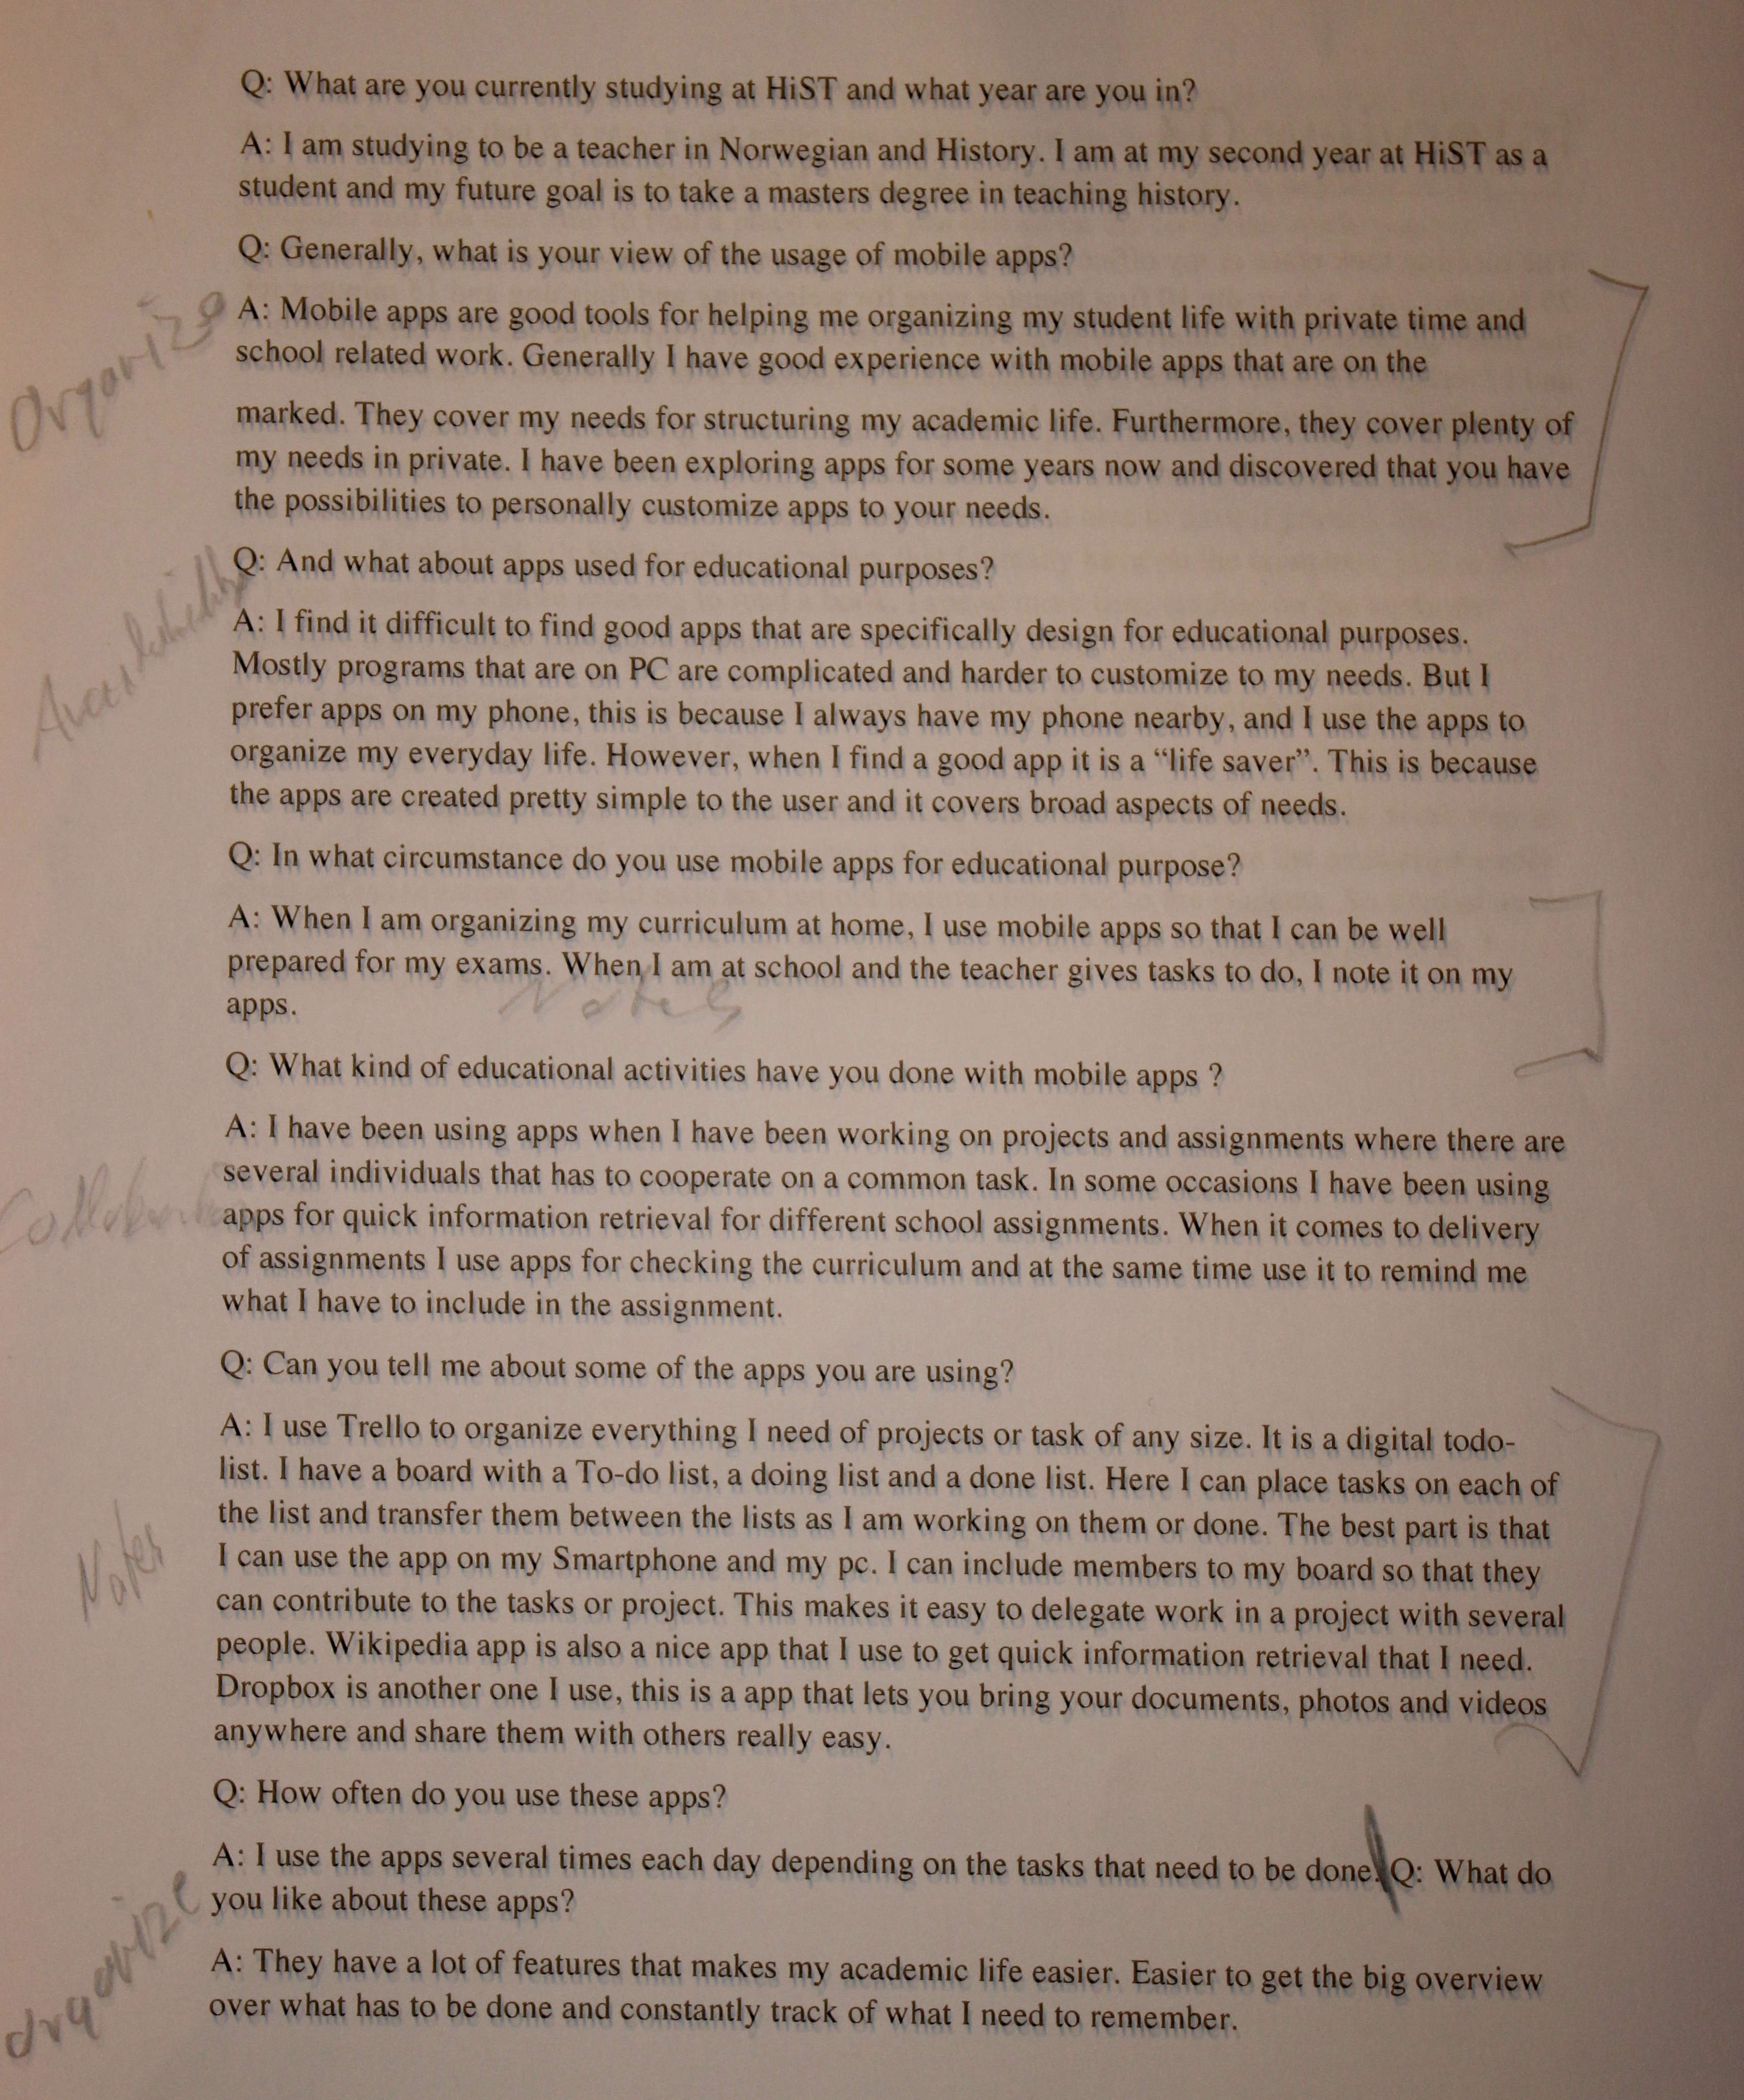
\includegraphics[width=\textwidth]{coding} 
    \label{fig:coding}
The figure shows how the coding of the data has been performed. 
\end{figure}

\section{Data Analysis} %2pages, 900 words
% Your analysis of the material, describing the most central concepts. This can
%include frequency of codes appearing in the material (interview transcripts or
%observation reports); description of concepts and how they are linked to the
%coded data material; description of the connection between concepts (if
%applicable).

In the figure we can see that the relevant passages of text is marked by a
bracket in the right margin. These blocks marks the paragraphs that are relevant for
the research questions. Categories was derived while reading, as I had no
existing theory to derive from. It was an inductive approach.  

The data consists of five interviews, one passive observation, and two
participant observations. The interviews, with questions, are planned and
scheduled beforehand. This gives all the interviews a consistency. Much of the
same information can be found in all the interviews. The one passive
observation distinguishes itself as being the only data collection of it's
type. Although, the data from this observation gives a perspective from the
other inputs. The passive observation contributes to a wider view. A more
distanced point of view that covers areas the two other methods provide don't. 
The participant observations are the most biased one, as the observer are
interacting with the subjects. Notes can also not be taken during the
observation, but has to be written down afterwords. This makes the observations
biased by the observer. Although the participant observations can enlighten the
use of mobile apps in interactions between people.  

\paragraph{Skimming} 
%- Initial reading of the materials. At first, you will skim though all of the data materials to get the main idea
After skimming through the data the main aspects are quite clear. Use of mobile
applications in education is the main theme of the data. Furthermore we have
some concepts that reoccur. The most reoccurring concepts are communication,
organization, and notes. 

\paragraph{Filtering} 
%- Intensive reading of the materials. Try to identify the segments of text that relevant to the research questions.
After filtering the text for useful sections it is obvious that there are few
sections of importance. Most questions give inconclusive clues of the data. 
The amount of data that does not contribute to the
enlightenment of the research questions is surprisingly large.  

\paragraph{Coding}
%: label the segment of text by some meaningful and structured words/terms
By coding the data we get some phrases, or codes, that repeats through the
data. The most significant ones are facebook, organize, notes, communication,
availability. The coding was done by the 'Open coding' way of analysing text. 
The codes indicates that the data is very focused on a small number of codes
and concepts. 

\paragraph{Identify concepts}
%: group the overlap/ similar or close codes into a higher-order label (concepts)
Concepts are derived from the codes. Similar and overlapping codes are combined
into a higher-order label. From the codes descried in the previous paragraph we
can see that it is difficult to find common traits among them. The codes can be
seen as concepts in themselves.   

\paragraph{Environment}
The environment for all observations were academically inspired. The interviews
had academicals as subjects, while the passive and participant, observations
were executed on campus in a setting related to education. 
The interviews have a closed environment, few distractions and a focused
atmosphere. Passive observations have the opposite atmosphere of interviews,
open and unfocused. Participant observations are somewhere in between the two. 

\paragraph{Observations}
The concepts are organised in table 1. From the table we can see the emphasised
concepts, and their frequency.  
 
Continuing with the description of the found markers, they range from
communication, the most observed concept,
to notes, which is the least observed concept. 

That communication is the most observed is not surprising. Communication is by
far the most common action among humans. On the other hand it is peculiar that
taking notes is the least common marker. One should think that students would
take more notes with mobile devices. 

The middle section with organize, facebook and availability comes in an
increasing frequency. All the concepts are common activities in daily life and
is to be expected of mobile app use. Again the distance to education is clearly
present. Or rather the lack of closeness, which indicates that further
observations might give indications of connections between app use and
education.

% basic table
% http://en.wikibooks.org/wiki/LaTeX/Tables
% the "{ l c r }" part decides if the content of a cell should be at the center,
% left or right. 
\begin{table}
\centering
\label{tbl:observations}
\caption{Observations. int=interview, p=passive observation, ap=participant observations}
\begin{tabular}{ l c |r |r |r |r |r |r |r |r } 
Concept & freq & int1 & int2 & int3 & int4 & int5 & p & ap1 & ap2 \\
\hline
facebook & 6 & * & * & & * & & * & * & *\\
organize & 4 & * &  & * & * & & & * & \\
notes & 3 & & & * & * & & * & &  \\
communication & 7 & * &  * & * & * & * & * & & * \\
availability & 5 & & * & * & * & * & & & * \\
\end{tabular}
\end{table}

\section{Self-reflection} %1page, 450 words
%presents your own reflection on the characteristics of data that you got from
%interview transcripts and observation reports; your experience on coding and
%identifying concepts; and your reflection on the application of knowledge from
%the course.

quantity and quality of data. 
The data set provided gives insight into app use on mobile devices. Although,
how much insight it gives into the relation between mobile apps and education
are up for discussion. 

The quantity of data is quite small to say something conclusive. Also, it is
not representative for the academic population. 
The passive observation session gives few data points as it is only
one observation. Which means we cannot say anything about the quality of the
observations while we have nothing to compare it to.
The participant observations have ok quality. It is as expected. In teamwork
one might not see lots of app use, which is ok. We should have had more
observations here to. I more observations would give more examples of use for
apps in group settings. 

Quality wise the data is ok. But it could have been better. 
The interviews in the dataset are badly structured and badly written down, hard to
read, and as a consequence hard to analyse. The interviews covers widely
different cases with different questions. The questions should have been the
same for all the datasets to be comparable. Passive observations in the dataset
are limited, and few. The amount of comments in the passive observations are
less than one every other minute. In a room with over 400 people it should be
easy to note different observations. As for the participant observations, the
setting might have been better. In the two observation sessions the number of
actual observations are few, which is odd. On a normal day one could observe
uses of mobile apps everywhere all the time. The participant observations seems
to biased as the recorded use of applications is so low. Also, the lack of diversity of
the used applications are interesting it's own way. Does it indicate that we
use a very limited spectrum of mobile apps?  

%1: In which circumstance student use mobile apps for educational purpose?
From the analysed data students only use mobile apps for taking notes. Most
other use is for communication and organisation, which can be considered a
personal day to day purpose. In regards to research question 1 we can note that
the use of mobile apps for educational purposes are very limited.  

%2: What kind of educational activities has been done with mobile apps?
Research question 2 asks what kind of educational activities apps were used for. The simple  
answer is only notes. The more complex and inconclusive answer is that mobile
apps are used in a variety of linked activities that to some extent has an
effect on educational activities. An example of this is email, it is for
example used to distribute curriculum and plan meetings. Another is facebook.
These days everyone uses facebook as a platform for collaboration and
communication. 

%3: What kind of impacts does mobile apps has on student academic life?
As for the impact apps have on the academic life, it is moderate. The impact of
mobile apps affect everyday life more than it does the academic life. This is
considering a definition of the academic life as aspects that has to do with
activities directly linked to campus or the university. Here the definition of
academic life is rather unsubstantial. It says nothing about the boundaries or
interpretations is has. As an example a person that is a student, but is never
on campus might use a wide array of different mobile apps, while a student that
visits campus every day might not use any mobile applications.  

In short summary the data is inconclusive and small. It should have been more
data, and it should have been better structured.
The research questions should be more precisely articulated, so that their
meaning and aim would be clearer.

The analysis in itself is also probably biased with personal impressions and
daily observations of mobile use.   

\end{document}
This is never printed
